\documentclass[letterpaper,11pt,twocolumn,twoside,]{pinp}

%% Some pieces required from the pandoc template
\providecommand{\tightlist}{%
  \setlength{\itemsep}{0pt}\setlength{\parskip}{0pt}}

% Use the lineno option to display guide line numbers if required.
% Note that the use of elements such as single-column equations
% may affect the guide line number alignment.

\usepackage[T1]{fontenc}
\usepackage[utf8]{inputenc}

% pinp change: the geometry package layout settings need to be set here, not in pinp.cls
\geometry{layoutsize={0.95588\paperwidth,0.98864\paperheight},%
  layouthoffset=0.02206\paperwidth, layoutvoffset=0.00568\paperheight}

\definecolor{pinpblue}{HTML}{185FAF}  % imagecolorpicker on blue for new R logo
\definecolor{pnasbluetext}{RGB}{101,0,0} %


\usepackage{wrapfig,subcaption,array,tabularx,multirow,caption} \usepackage[utf8]{inputenc}
\usepackage{booktabs}
\usepackage{longtable}
\usepackage{array}
\usepackage{multirow}
\usepackage{wrapfig}
\usepackage{float}
\usepackage{colortbl}
\usepackage{pdflscape}
\usepackage{tabu}
\usepackage{threeparttable}
\usepackage{threeparttablex}
\usepackage[normalem]{ulem}
\usepackage{makecell}

\title{DATA2X02 Group Assignment}

\author[a]{Group: W13A Early 8}


\setcounter{secnumdepth}{3}

% Please give the surname of the lead author for the running footer
\leadauthor{}

% Keywords are not mandatory, but authors are strongly encouraged to provide them. If provided, please include two to five keywords, separated by the pipe symbol, e.g:
 

\begin{abstract}

\end{abstract}

\dates{This version was compiled on \today} 

% initially we use doi so keep for backwards compatibility
% new name is doi_footer

\pinpfootercontents{DATA2X02 Group Assignment}

\begin{document}

% Optional adjustment to line up main text (after abstract) of first page with line numbers, when using both lineno and twocolumn options.
% You should only change this length when you've finalised the article contents.
\verticaladjustment{-2pt}

\maketitle
\thispagestyle{firststyle}
\ifthenelse{\boolean{shortarticle}}{\ifthenelse{\boolean{singlecolumn}}{\abscontentformatted}{\abscontent}}{}

% If your first paragraph (i.e. with the \dropcap) contains a list environment (quote, quotation, theorem, definition, enumerate, itemize...), the line after the list may have some extra indentation. If this is the case, add \parshape=0 to the end of the list environment.


\captionsetup[figure]{labelfont={it,bf,scriptsize},textfont={it,scriptsize},labelsep=colon}
\captionsetup[table]{labelfont={it,bf,scriptsize},textfont={it,scriptsize},labelsep=colon}
\captionsetup[FLOAT_TYPE]{labelformat=simple, labelsep=colon}

\vspace{-20truemm}

\hypertarget{abstract}{%
\section{Abstract}\label{abstract}}

We aim to test the importance of alcohol content as a significant
predictor of red and white wine quality in a dataset containing the
physicochemical tests of red and white wine. This was measured by
comparing the \(R^{2}\) in a simple linear regression (SLR), containing
only alcohol content and quality, to a multi-linear regression (MLR).
The MLR was built through stepwise model selection, using inputs with a
correlation of greater than 0.2 with wine quality. The results show that
alcohol content is both significant and the most important predictor of
red and white wine quality(p-value less than 0.001) as the there was
only a 7-11\% increase in the MLR \(R^{2}\) compared to the SLR
\(R^{2}\) (19-23\%).

\hypertarget{introduction-and-data-exploration}{%
\section{Introduction and data
exploration}\label{introduction-and-data-exploration}}

We observed 12 variables, 11 independent continuous variables and 1
dependent discrete variable, which were produced as a result of
physicochemical tests performed on red and white wine from Portugal. The
data also did not include useful variables such as brand, grape type or
price. The data set was acquired from the University of California,
Irvine. The data had a far larger number of observations for white wine
compared to red. Additionally, most of the quality results were medium
quality with few being low or high. This was measured between 1 -- 10,
with 10 being of higher quality.

On observation, alcohol(vol\%) has the strongest correlation of 0.44 and
0.48 for white and red wine respectively. This prompted us to wonder
\textbf{the extent to which alcohol content is the most important
predictor for wine quality?}

\hypertarget{analysis}{%
\section{Analysis}\label{analysis}}

\hypertarget{linear-regression-model}{%
\subsection{Linear Regression Model}\label{linear-regression-model}}

Investigating this by modelling a simple linear regression of alcohol
against quality gave an \(R^{2}\) value of 0.19 for white wine and 0.23
for red wine. This shows that 19\% of the variability in white wine and
23\% of the variability in red wine can be explained by the change in
alcohol. Additionally, both white and red wine show p-values that are
low enough to reject the null hypothesis (less than 0.001), suggesting
the slope parameter is statistically significant for both wines.

\begin{table}[h]
\begin{tabular}{ ccc } 
\hline
\textbf{} & \textbf{$R^2$} & \textbf{Adjusted $R^2$} \\
\hline
\textbf{White} & 0.1897 & 0.1896 \\ 
\textbf{Red} & 0.2267 & 0.2263 \\
\hline
\end{tabular}
\centering
\caption{Summarize goodness of fit of SLR models.}
\label{table:performance_slr}
\end{table}

\vspace{-6truemm}

In order to measure the extent that alcohol influences wine quality we
build a multiple regression model for each wine to measure the change in
\(R^{2}\) as we add new predictors. Care was taken to ensure all
predictors are linearly correlated with the response variable, quality.
Violations of linearity can result in a systematic error and may
seriously hinder the quality of our models' predictions. Taking the most
correlated variables for white gives chlorides, volatile acidity,
density and fixed acidity while for red we have citric acid, volatile
acidity and sulphates. This can be seen in the shiny app whose link is
provided in the appendix.

\hypertarget{model-interpretation}{%
\subsection{Model interpretation}\label{model-interpretation}}

The multi-linear regression models were built using forward and reverse
stepwise selection for both datasets. In both cases, the red and white
wine models were found to be identical. This evidence suggests that
these models are robust and are suitable for use in our analysis.

The red wine model incorporates sulphates, alcohol and volatile acidity,
with a equation of \[quality=2.61+0.31(alcohol)-1.22(volatile~acidity)\]
\vspace{-8truemm} \[+0.68(sulphates)+\epsilon.\]

All variables included in the model have highly significant p-values
less than 0.001. Showing in table \ref{table:performance_mlr}, the
\(R^{2}\) and \(R^{2}\) adjusted of 0.336 and 0.335 were observed
respectively.

More variables were found useful in constructing the white wine, with a
equation of \[quality= -47.65 + 0.4(alcohol)-2.09(volatile\_acidity)\]
\vspace{-8truemm}
\[+ 50.91(density) -0.1(fixed\_acidity) -1.32(chlorides)+\epsilon.\]
This is potentially a result of the increased sample size. Within the
white wine dataset, alcohol, volatile acidity, density, fixed acidity
and chlorides were found to be significant, where chlorides had a
p-value of 0.014 with all other variables measuring below 0.001. As
shown in table \ref{table:performance_mlr}, the model produced an
\(R^{2}\) and \(R^{2}\) adjusted values of 0.256 and 0.255 respectively.

The estimate for density was very large compared to the other variables
to account for the low mean and variation in the values. Density has a
positive estimate in the model despite its correlation with quality
being negative. This is likely due to interlinearity between the
independent variables, which can lead to an estimate of opposite sign to
the correlation coefficient.

\begin{table}[ht]
\begin{tabular}{ ccc } 
\hline
\textbf{} & \textbf{$R^2$} & \textbf{Adjusted $R^2$} \\
\hline
\textbf{White} & 0.2561 & 0.2554 \\
\textbf{Red} & 0.3359 & 0.3346 \\
\hline
\end{tabular}
\centering
\caption{Summarize goodness of fit of MLR models.}
\label{table:performance_mlr}
\end{table}

\vspace{-8truemm}

\hypertarget{assumption-checking}{%
\subsection{Assumption checking}\label{assumption-checking}}

Despite moderately weak linear relationships between predictors and wine
quality, there is a lack of patterns in the residual plots, excluding
striations which occur from measuring the discrete `quality' variable,
reinforcing an approximately linear relationship. Furthermore, the
assumption for independence is satisfied as physicochemical tests are
measured separately for each bottle of wine. The residual plot figure
\ref{fig:red_resid} shows equal variance among red wine residuals but
slight patterns of heteroskedasticity in white wine residuals showing by
figure \ref{fig:white_resid}. Hence, heteroskedasticity corrected
standard errors were used to compute p-values. This resulted in all
converted p-values measuring below 0.001,including `Chlorides'. Despite
slight deviations in the lower tails, residuals largely followed the
QQ-line. Additionally with the large number of observations we can rely
on the central limit theorem to satisfy the normality assumption.

\hypertarget{performance-evaluation}{%
\subsection{Performance evaluation}\label{performance-evaluation}}

A 10 fold cross validation test was conducted to measure out-of sample
model performance. The \(R^2\) values indicate 26\% and 34\% of the
observations can be explained from white and red wine models, indicating
poor insample performance. Further, the RMSE values show on average the
predicted quality of white and red wine differed from actual quality by
0.76 and 0.66 respectively. Given rounding, this results in a constant
one level difference in our predicted values, indicating fairly poor
model performance. Thus, predicted values should be interpreted with
care.

\hypertarget{results}{%
\section{Results}\label{results}}

A 10 fold cross validation test was conducted to measure out-of sample
model performance, giving the results from table
\ref{table:performance_sum}. The \(R^{2}\) values indicate 26\% and 34\%
of the observations can be explained from white and red wine models,
indicating poor out of sample performance. Further, the RMSE values show
on average the predicted quality of white and red wine differed from
actual quality by 0.76 and 0.66 respectively. Given rounding, this
results in a constant one level difference in our predicted values,
indicating fairly poor model performance. Suggesting predicted values
should be interpreted with care.

\begin{table}[h]
\begin{tabular}{ ccccccc } 
\hline
\textbf{} &  \textbf{RMSE} & \textbf{$R^2$} & \textbf{MAE} & \textbf{RMSESD} & \text{$R^2$SD} & \textbf{MAESD}\\
\hline
\textbf{SLR White} & 0.80 & 0.19 &  0.63 &  0.02    & 0.04  & 0.02 \\
\textbf{SLR Red} & 0.71 &   0.23 &  0.56 &  0.05    & 0.07  & 0.04 \\
\textbf{MLR White} & 0.76 & 0.26    & 0.60  & 0.03  & 0.03 & 0.02 \\
\textbf{MLR Red} & 0.66 &   0.34 & 0.52 & 0.03  & 0.06 &    0.02 \\
\hline
\end{tabular}
\centering
\caption{Summarize performance of models.}
\label{table:performance_sum}
\end{table}

\vspace{-6truemm}

Alcohol appears to be a significant predictor in both red and white wine
models with a p-value less than 0.001. For a 1 unit increase in alcohol,
there is an increase of 0.31 in white and 0.40 in red quality. As
alcohol content explains 19\% (red) and 23\% (white) of the simple
linear model, with only a 7-11\% increase in explanatory power for
adding additional variables in the multilinear model, this implies
alcohol content is the most influential predictor in determining the
quality of red and white wine.

\hypertarget{discussion-and-conclusion}{%
\section{Discussion and conclusion}\label{discussion-and-conclusion}}

Although models developed are proven to be significant, there have been
several limitations. The differing number of observations between red
and white wine resulted in inconsistent variances of data, which can
impact the quality of inferences. However, as we are focused on
comparing the \(R^2\) values instead of estimating predictions, this is
less of a concern. If grapes are from the same batch, the assumption of
independence could be violated, making the inference of results
unreliable. In addition, variables are not necessarily linear as the
highest correlation coefficient with wine quality measured 0.48. Hence,
as supported by Cortez (2019), MLR is the worst model for predicting
wine quality for this dataset. Future studies may focus on wine quality
predictions by evaluating alternative machine learning techniques such
as K-nearest neighbor and random forest which are able to capture
non-linearity.

\newpage

\hypertarget{references}{%
\section{References}\label{references}}

\begin{itemize}
\tightlist
\item
  P. Cortez, A. Cerdeira, F. Almeida, T. Matos and J. Reis. Modeling
  wine preferences by data mining from physicochemical properties. In
  Decision Support Systems, Elsevier, 47(4):547-553, 2009.
\item
  Alboukadel Kassambara (2020). ggpubr: `ggplot2' Based Publication
  Ready Plots. R package version 0.4.0.
  \url{https://CRAN.R-project.org/package=ggpubr}
\item
  Hao Zhu (2020). kableExtra: Construct Complex Table with 'kable'and
  Pipe Syntax. R package version 1.3.1.
  \url{https://CRAN.R-project.org/package=kableExtra}
\item
  Yuan Tang, Masaaki Horikoshi, and Wenxuan Li. ``ggfortify: Unified
  Interface to Visualize Statistical Result of Popular R Packages.'' The
  R Journal 8.2 (2016): 478-489.
\item
  Max Kuhn (2020). caret: Classification and Regression Training. R
  package version 6.0-86. \url{https://CRAN.R-project.org/package=caret}
\item
  Wickham et al., (2019). Welcome to the tidyverse. Journal of Open
  Source Software, 4(43), 1686,
  \url{https://doi.org/10.21105/joss.01686}
\end{itemize}

\hypertarget{appendix}{%
\section{Appendix}\label{appendix}}

\begin{figure}[H]

{\centering 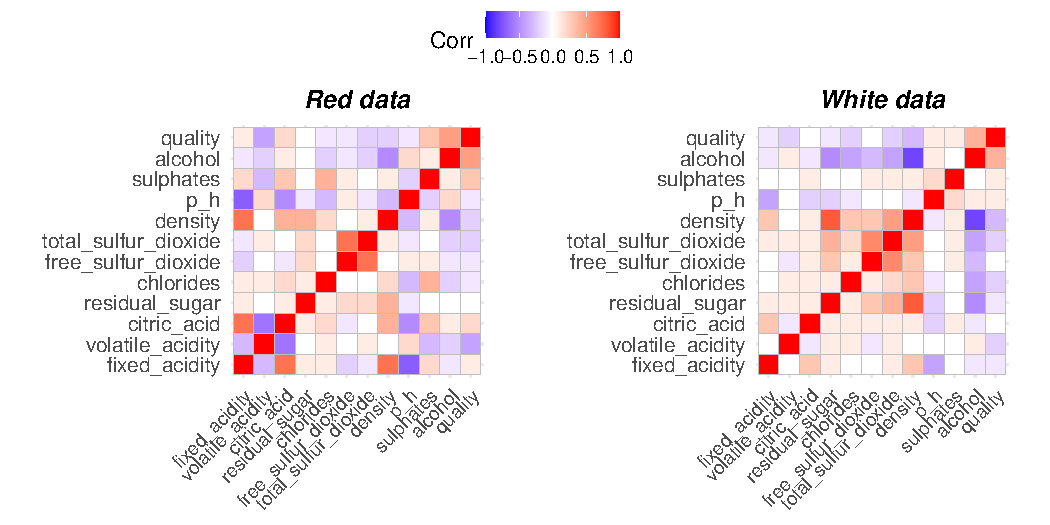
\includegraphics{DATA2X02_group_files/figure-latex/unnamed-chunk-8-1} 

}

\caption{Correlation matrices for red and white wine data. The correlation metric is the Pearson's correlatin coefficients.}\label{fig:unnamed-chunk-8}
\end{figure}

\begin{figure}[H]

{\centering 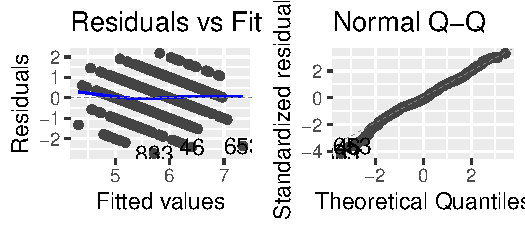
\includegraphics{DATA2X02_group_files/figure-latex/red_resid-1} 

}

\caption{Residual plot and normal Q-Q plot of the stepwise regression model for red wine data.}\label{fig:red_resid}
\end{figure}

\begin{figure}[H]

{\centering 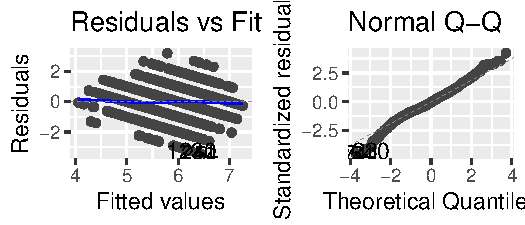
\includegraphics{DATA2X02_group_files/figure-latex/white_resid-1} 

}

\caption{Residual plot and normal Q-Q plot of the stepwise regression model for white wine data.}\label{fig:white_resid}
\end{figure}

\textbf{Shiny app:}
\url{https://stephan-iie.shinyapps.io/Linearity/?_ga=2.34896929.1856433187.1605152041-1797514058.1605152041}

%\showmatmethods


\bibliography{pinp}
\bibliographystyle{jss}



\end{document}

